\documentclass[10pt,conference,compsocconf]{IEEEtran}

\usepackage{hyperref}
\usepackage{graphicx}
\usepackage{xcolor}
\usepackage{blindtext, amsmath, comment, subfig, epsfig }
\usepackage{grffile}
\usepackage{caption}
%\usepackage{subcaption}
\usepackage{algorithmic}
\usepackage[utf8]{inputenc}


\title{CS-523 SecretStroll Report}
\author{Wicky Simon, Nunes Silva Daniel Filipe}
\date{April 2020}

\begin{document}

\maketitle

\begin{abstract}
    %Please report your design, implementation details, and findings of the second project in this report. \\
    %THE REPORT SHOULD NOT EXCEED 5 PAGES.
    This project consists of three parts, all related to a central topic : Privacy in a location based service.
    The first part makes use of Attributes based credentials (ABC) and zero-knowledge proof to anonymously query a server for nearby Points of Interests (PoIs), while proving the ownership of a subscription. The second part we evaluate the loss of privacy induced by IP-level metadata. The last part of this project is dedicated to trying to infer location of query author, based solely on metadata. 
\end{abstract}

\section{Introduction}

The aim of the first part of this project is to build a privacy-friendly location based service, SecretStroll, which allows users to query a database about nearby PoIs while remaining anonymous. Since this service is not free, every query must provide the proof of an active subscription. Each PoIs is part of a category such as \textit{Restaurant}, \textit{Cinema}, \textit{Train station}, etc. Each of these category are part of a subscription and a user can have many of them, which naturally leads to ABC. A user joining the service first register himself with the category he paid for and then sign each of his query anonymously, revealing only the categories he want to get PoIs from.
%Second part 
%Thirs part

\section{Attribute-based credential}
The base of the ABC scheme for this work is described in Section 6 of \cite{PS_Scheme}. This scheme has been used as follows : 
\begin{itemize}
    \item The messages mentionned in \cite{PS_Scheme} are attributes, representing categories of PoIs. The server creates a public key large enough to encode all of these attributes. 
    \item When a user wants to register, she commits to attributes she paid for, that will remain hidden. She uses a zero-knowledge proof (ZKP) to prove that she did so correctly. The server checks the proof, and sign this commitment that she will then use as credential.
    \item When a user makes a query, she choose the attributes (i.e the categories of PoIs) that she want. She then makes use of her credential to prove she has a subscription for the queried attributes, using a ZKP. She also uses this credential to sign a message representing her current location using the Fiat-Shamir heuristic described in \cite{FSheuristic} and detailed later.
\end{itemize}

In order to make the ZKP non-interactive, we use the Fiat-Shamir heuristic. The challenge that the prover would send is replaced by a cryptographic hash of all known values. During the registration, the challenge is composed of the committed attributes, the commitment used for the ZKP and the server's public. To sign the message for a query, it is simply added to the other values constituting the challenge. 

This overall approach leaks only the number of attributes chosen, but it is necessery for the server to correctly compute the ZKP. Otherwise, hidden attributes cannot be inferred and every credential is unique.

\subsection{Test}
The system is tested with six different tests : 
\begin{enumerate}
    \item \textit{test\_generate\_ca()} : The server's certificate generation is tested with a simple structure test, to see if all keys have the right lenghth.
    \item \textit{test\_credentials\_difference()} : Two requests are created with the same input parameters, a registration is perforemd with both of them and two credentials are created. To preserve anonymity, the requests and the built credential should be different. \\ Two credentials created from the same request should also be different.
    \item \textit{test\_tampered\_credential()} : A request with invalid credential should be rejected. In this test, a valid credential is tampered to be invalid.
    \item \textit{test\_correct\_credential()} : A request with a correct credential should be accepted.
    \item \textit{test\_correct\_credential\_no\_attributes()} : A request revealing no attributes should be valid.
    \item \textit{test\_wrong\_revealed\_attr()} : A request revealing unobtained attributes should be invalid.
\end{enumerate}
The effectiveness of these tests could be assessed using a standard metric such as branch coverage or coverage. However, these metrics are not complete and will not discover every bug present in the code.


\subsection{Evaluation}
Evaluate your ABC: report communication and computation stats (mean and standard
deviation). Report statistic on key generation, issuance, signing, and
verification.

The system is benchmarked in two parts, an offline part, which evaluate pure computationnal time and an online part which evaluate the communication time.

\subsubsection{Offline benchmark}
The offline benchmark tests four features :
\begin{itemize}
    \item Key generation
    \item Credential issuance
    \item Message signing
    \item Signature verification
\end{itemize}
The result are shown in figure \ref{benchoffline_fig}
and reported in table \ref{benchoffline}
\begin{table}
\begin{tabular}{|c|c|c|c|}
    \hline
                            & Rounds  & Mean      & Std. deviation  \\
    \hline
    Key generation          & 1000    & 27.30 ms  & 4.30 ms         \\
    \hline
    Credential issuance     & 1000    & 41.86 ms  & 8.24 ms         \\
    \hline
    Message signing         & 1000    & 44.34 ms  & 10.32 ms        \\
    \hline
    Signature verification  & 1000    & 44.31 ms  & 9.52 ms         \\
    \hline    
\end{tabular}
\caption{Result of the offline benchmark, }
\label{benchoffline}
\end{table}
\begin{figure}
    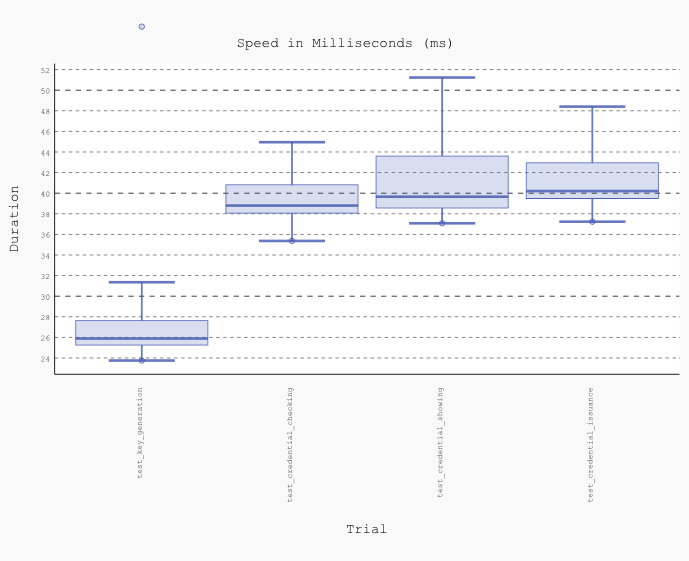
\includegraphics[width=\columnwidth]{benchmark.png} 
    \caption{Histogram of the offline benchmark}
    \label{benchoffline_fig}
\end{figure}

\subsubsection{Online benchmark}
The onlin benchmark tests two features :
\begin{itemize}
    \item Registration
    \item PoIs request
\end{itemize}
Note : This benchmark has requirements. Follow the instructions at the beginning of \textit{benchmark\_net.py}.

The result are shown in figure \ref{benchonline_fig}
and reported in table \ref{benchonline}
\begin{table}
\begin{tabular}{|c|c|c|c|}
    \hline
                    & Rounds    & Mean      & Std. deviation    \\
    \hline
    Registration    & 1000      & 53.58 ms  & 1.93 ms           \\
    \hline
    PoIs request    & 1000      & 90.07 ms  & 1.90 ms           \\
    \hline   
\end{tabular}
\caption{Result of the online benchmark}
\label{benchonline}
\end{table}
\begin{figure}
    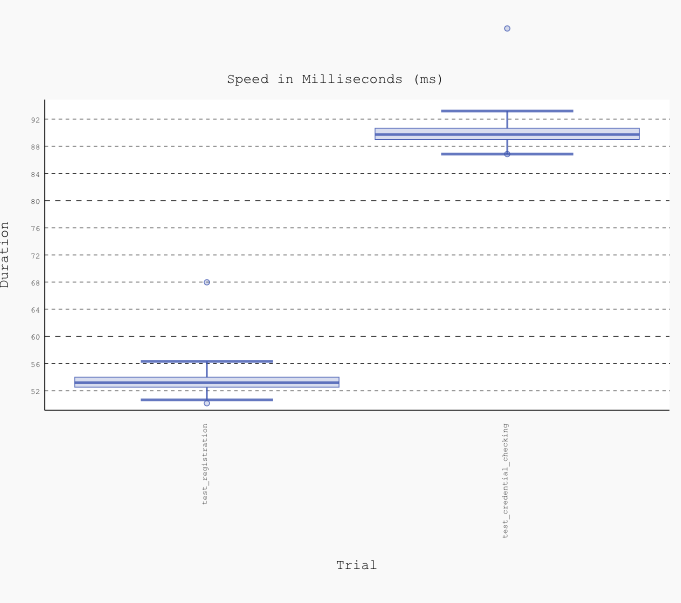
\includegraphics[width=\columnwidth]{benchmark_net.png}
    \caption{Histogram of the online benchmark}
    \label{benchonline_fig}
\end{figure}


\section{(De)Anonymization of User Trajectories}

\subsection{Privacy Evaluation}
We evaluate the privacy risks using simulated data of two hundred users who made use of the application hundred times each in average over twenty days. We assume that no mechanism to hide any kind of data is used, i.e. data is sent in cleartext inside standard IP packets. Any malicious adversary could hack the application servers or sniff the network between a user and the server in order to retrieve similar datasets which include IP addresses, locations, query types, timestamps and responses. According to \cite{dont}, the IP address or a set or IP addresses are relevant attributes because they can be linked to a given user since they are persistent for a certain duration. Moreover, combining IP addresses with location and time data makes sense since users often keep their habits that they may share with very few people \cite{on}, i.e. they may work during the day at their office, be back home in the evening and do an activity at some specific location. Therefore, we expect this implementation to leak senstive informations about the users. As a proof of concept for breaching users privacy, we to infer work and home locations of users as well as habits in their activities.

We build our attacks in a constructive way, starting by learning general tendencies about the users, then, we focus on one specific user in order to learn how far we can go with breaching breach its privacy.

As stated before, home and work are sensitive locations because they allow to identify users. In order to learn about them, we go through all users queries and check if users queries locations correspond to home types locations such as \textit{appartment blocks} or \textit{villas} as well as work types locations such as \textit{offices}, \textit{laboratories} or \textit{companies}. It turns out that each user has one location of each from where it does the majority of its queries which allows us to draw a map linking IP addresses to their corresponding home and work locations. Moreover, \ref{share_fig} confirms our concern about users anonymity once their home and work locations would leak in the given setup. The logarithmic scale clearifies the orders of magnitude between people who share or not these POIs showing that the majority of the users have a tuple home and work location that they share with very few people as presented in \cite{on}.

\begin{figure}
  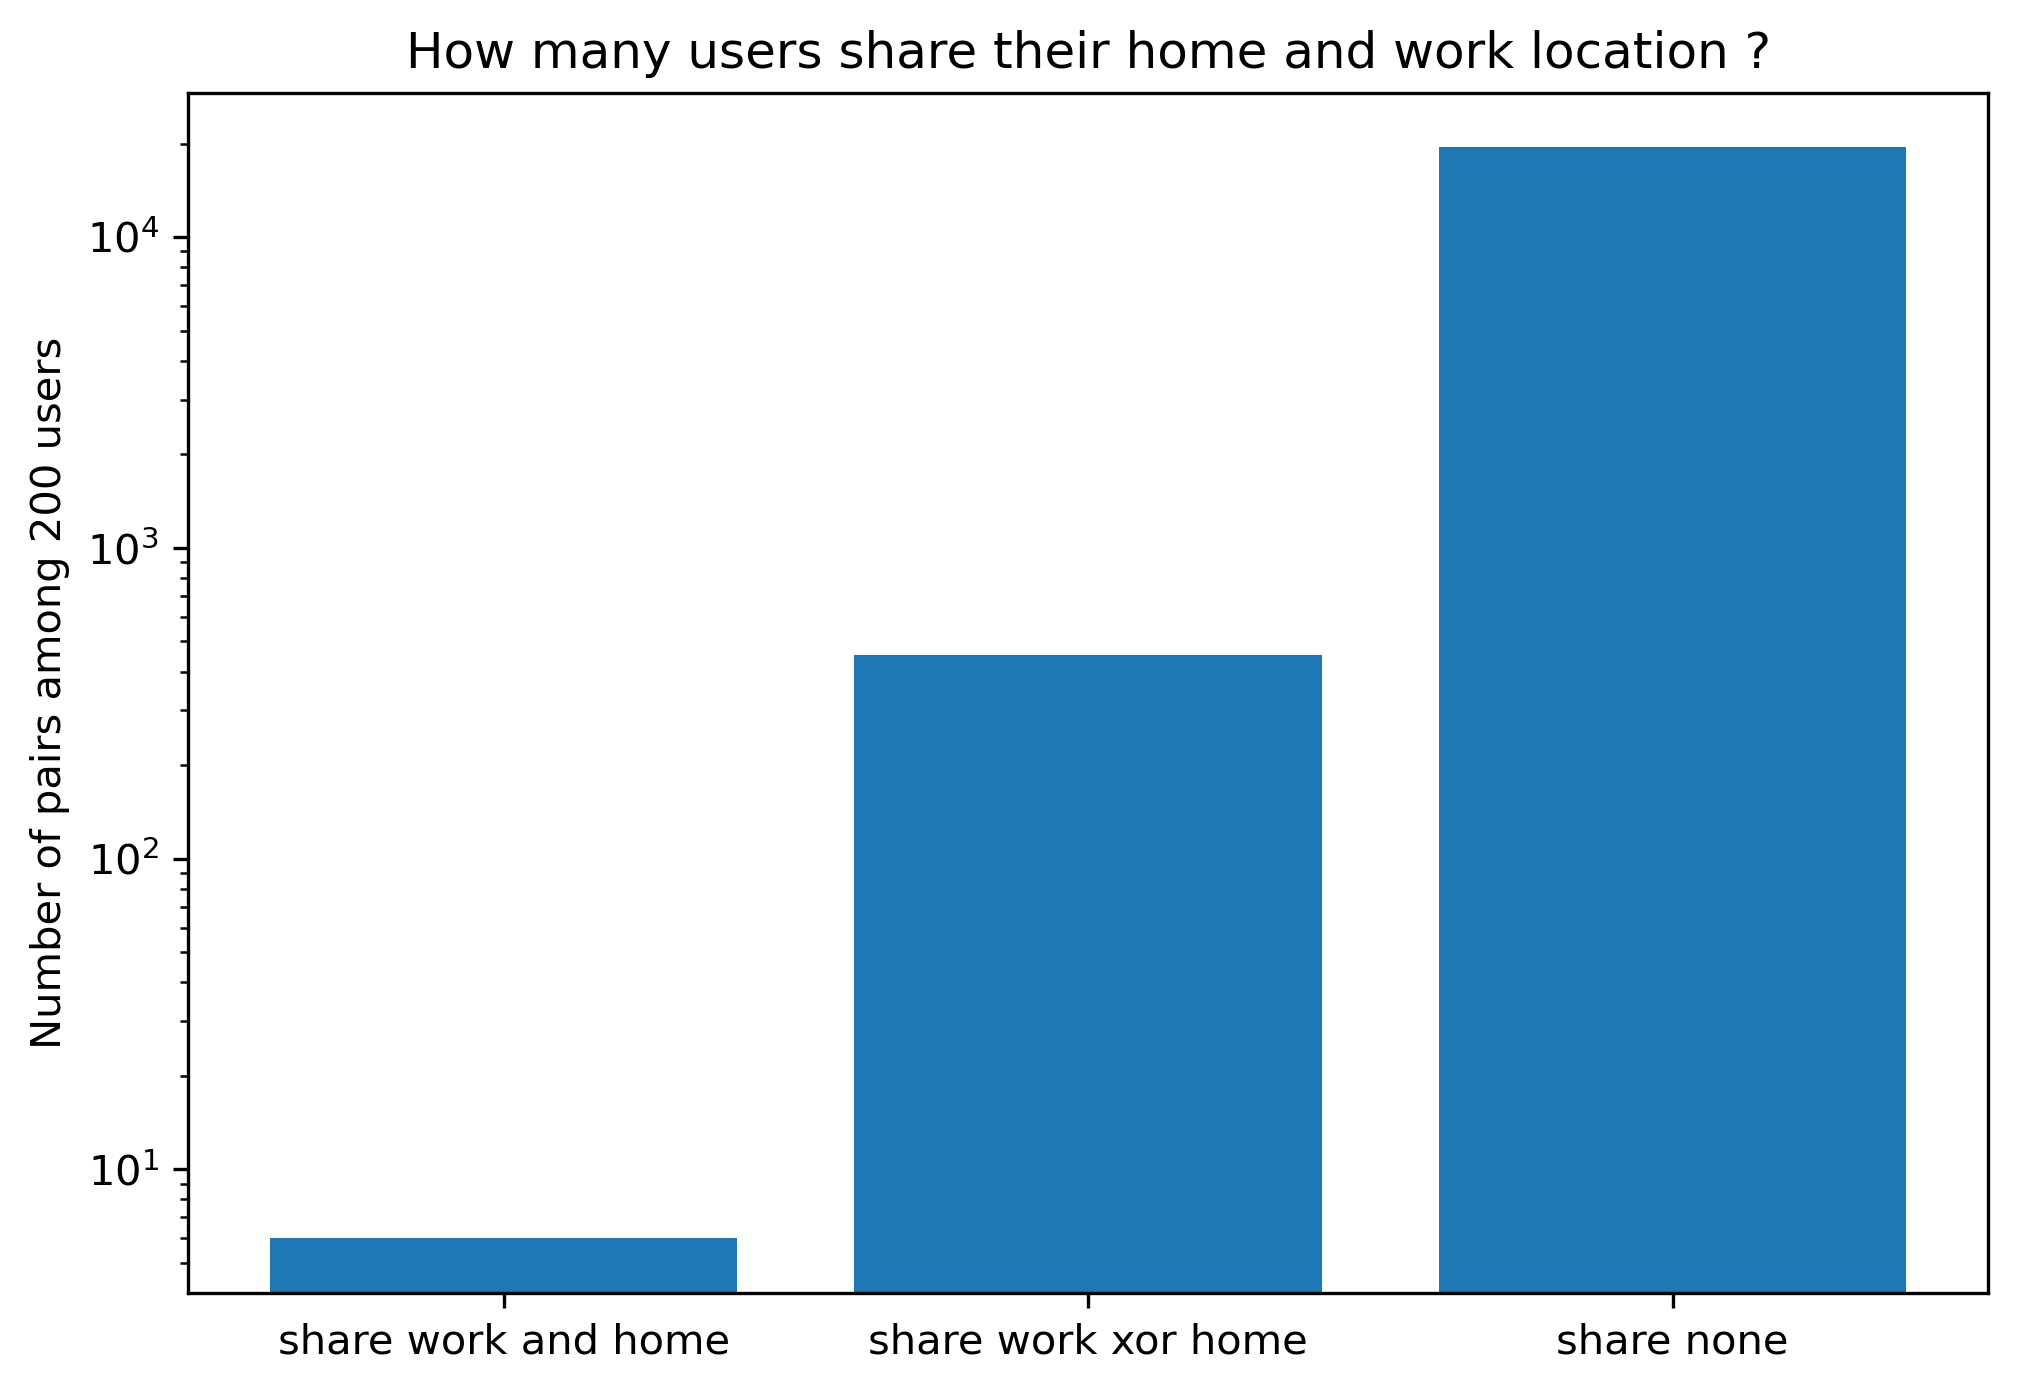
\includegraphics[width=\columnwidth]{share.png}
  \caption{Comparison of how people share their main POIs}
  \label{share_fig}
\end{figure}

Then, we analyze when users make use of the app from their home and work locations. On the one hand, we observe that they use it regularly on a daily basis from home. On the other hand, we can see that they query the service from their work location only during weekdays, which is compatible with not being on their work location on the weekend. Moreover, we consider when the app is used during the day on weekdays in \ref{when_fig}. This shows that users likely spend their day at work while being at home at the end of the day. This short analysis gives a great understanding of users habits even though the presented results seem trivial.

\begin{figure}
  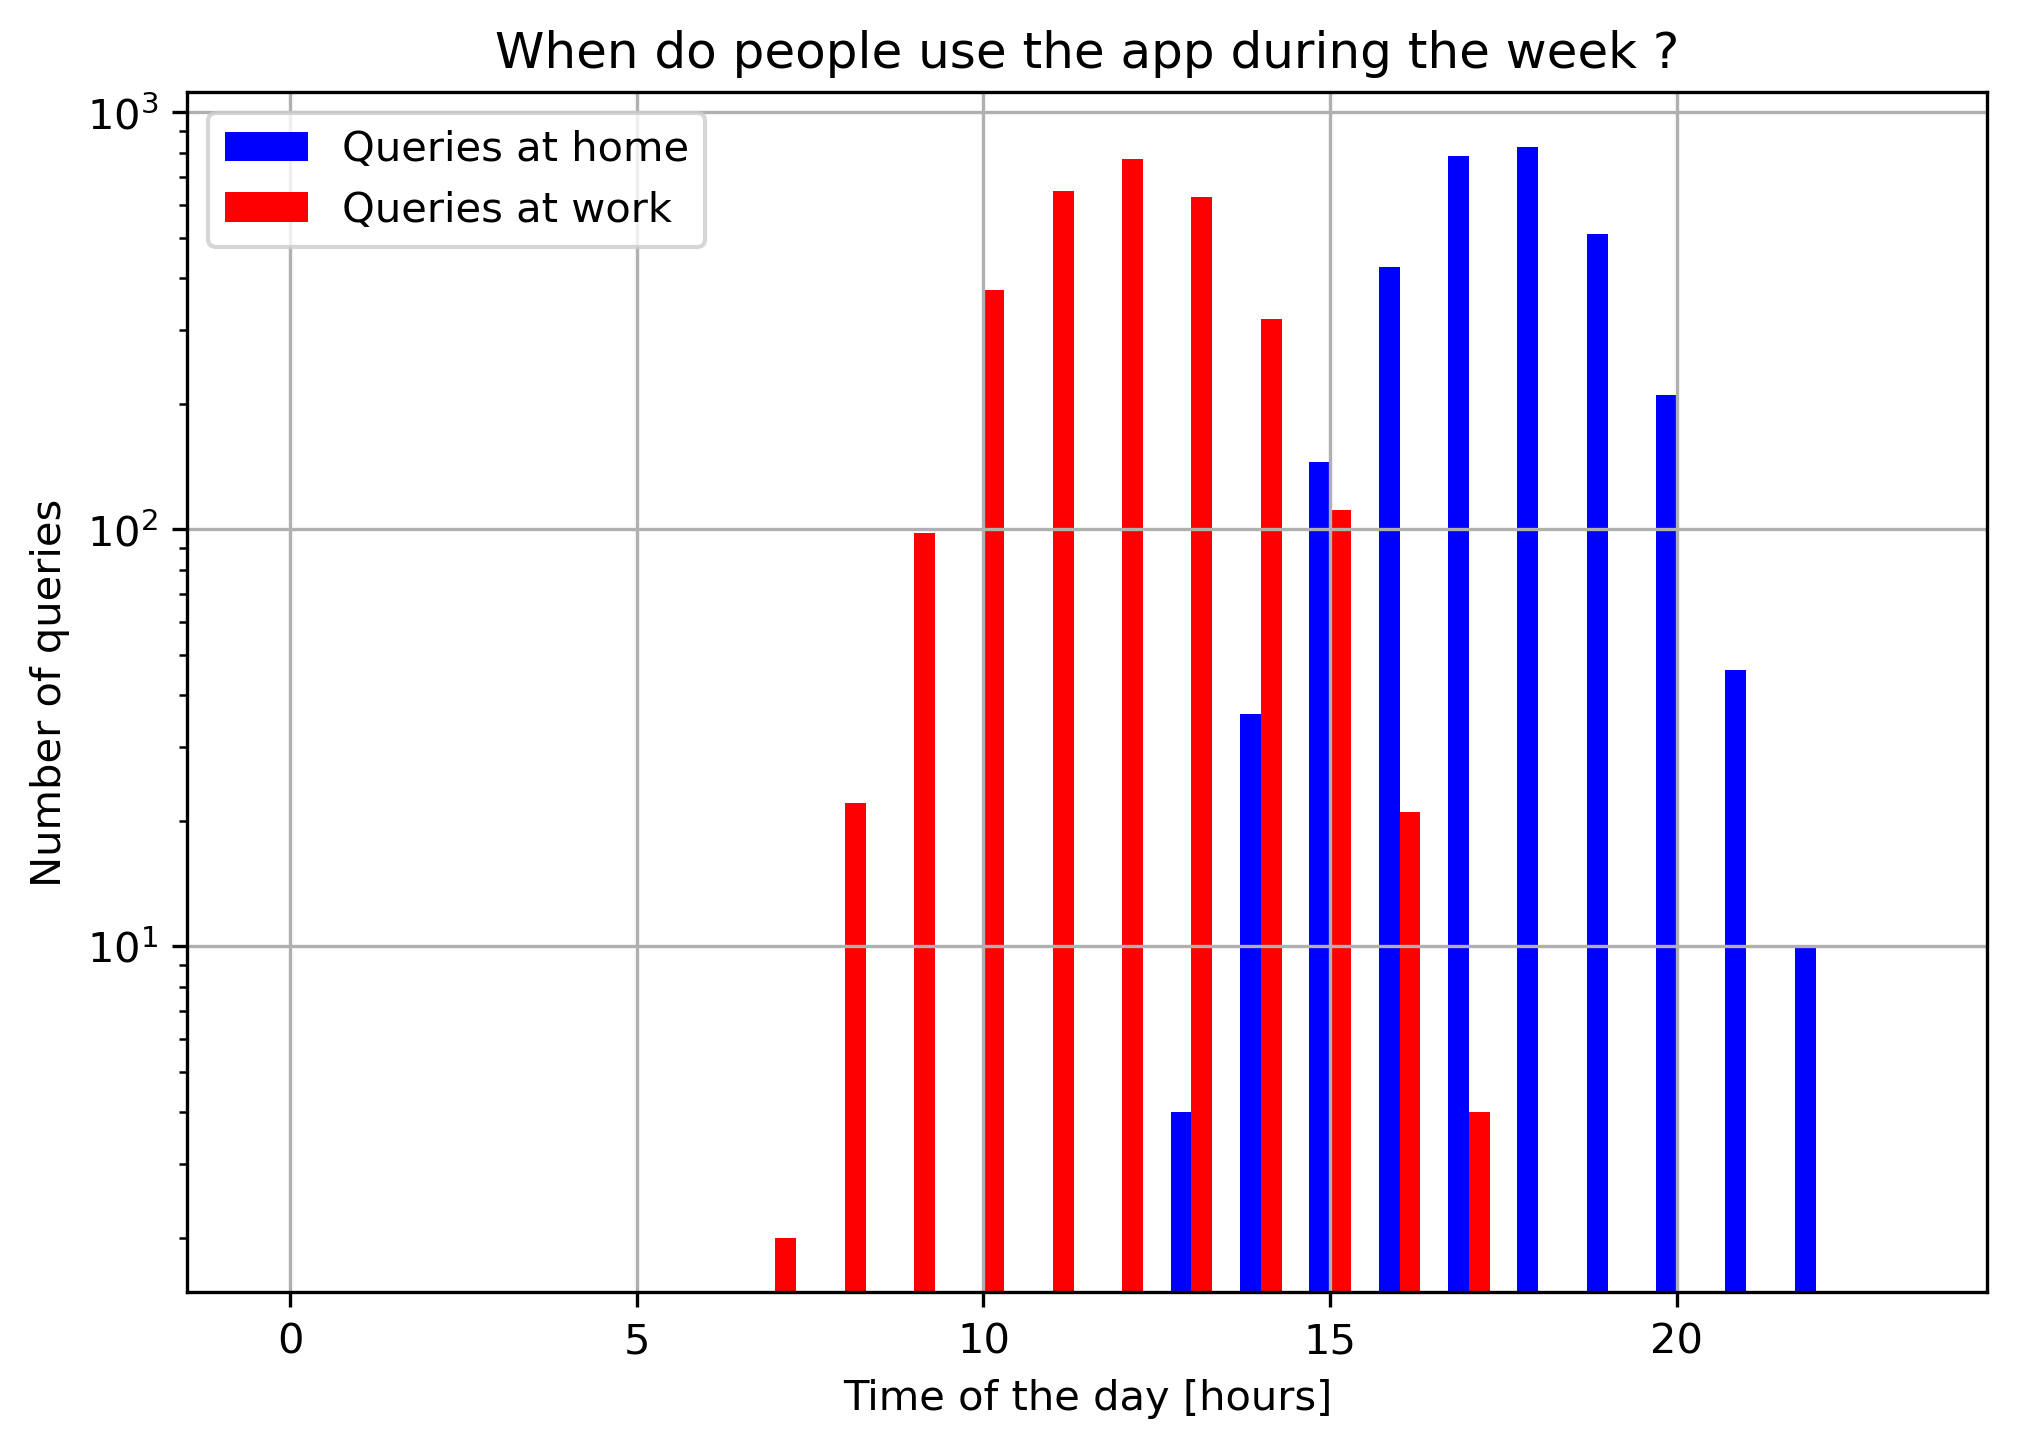
\includegraphics[width=\columnwidth]{when.png}
  \caption{User habits}
  \label{when_fig}
\end{figure}

Finally, we focus on breaching privacy of a chosen user to assess if we can learn more about a given user than general tendencies. Our results are condensed in the graph presented in \ref{random_fig} that shows how user moves as a function of time. We are able to determine where the user lives and works making use of our previous findings. From that, we can see how this user's life is centered around its home and work locations. In fact, it goes back and forth its home and work during the week while its trajectory take completely different paths on the weekends. Applying similar techniques for other POIs types allows us to learn about this user's favorite restaurant and when it used to eat there. Then, grouping \textit{bars} and \textit{clubs} as entertaining activities opposed to \textit{gym} and \textit{dojo} which can be considered quiet ones, we deduce that this particular user is more into the former ones which are located close to its home. He basically goes to the gym on the weekends as we can see these spiky outliers in \ref{random_fig}.

To sum up, we assessed how we could breach users privacy by analyzing either general habits about the users or more personal ones by focusing on specific users. This lead us to conclusive results regarding our initial references and expectations leveraging simple algorithms such as matching users queries locations with meaningful POIs. Cost would depend how close and severely someone wants to attack a specific user. As we shown, either we can keep it very general to learn about tendencies or focus on a given user. For future attack, we may be interested to evaluate how the current POIs locations may be related to the next queries that may allow us to understand better users behaviour. For example, how likely is it that a user wants to go for a beer after work compared to after gym ?

\begin{figure}
  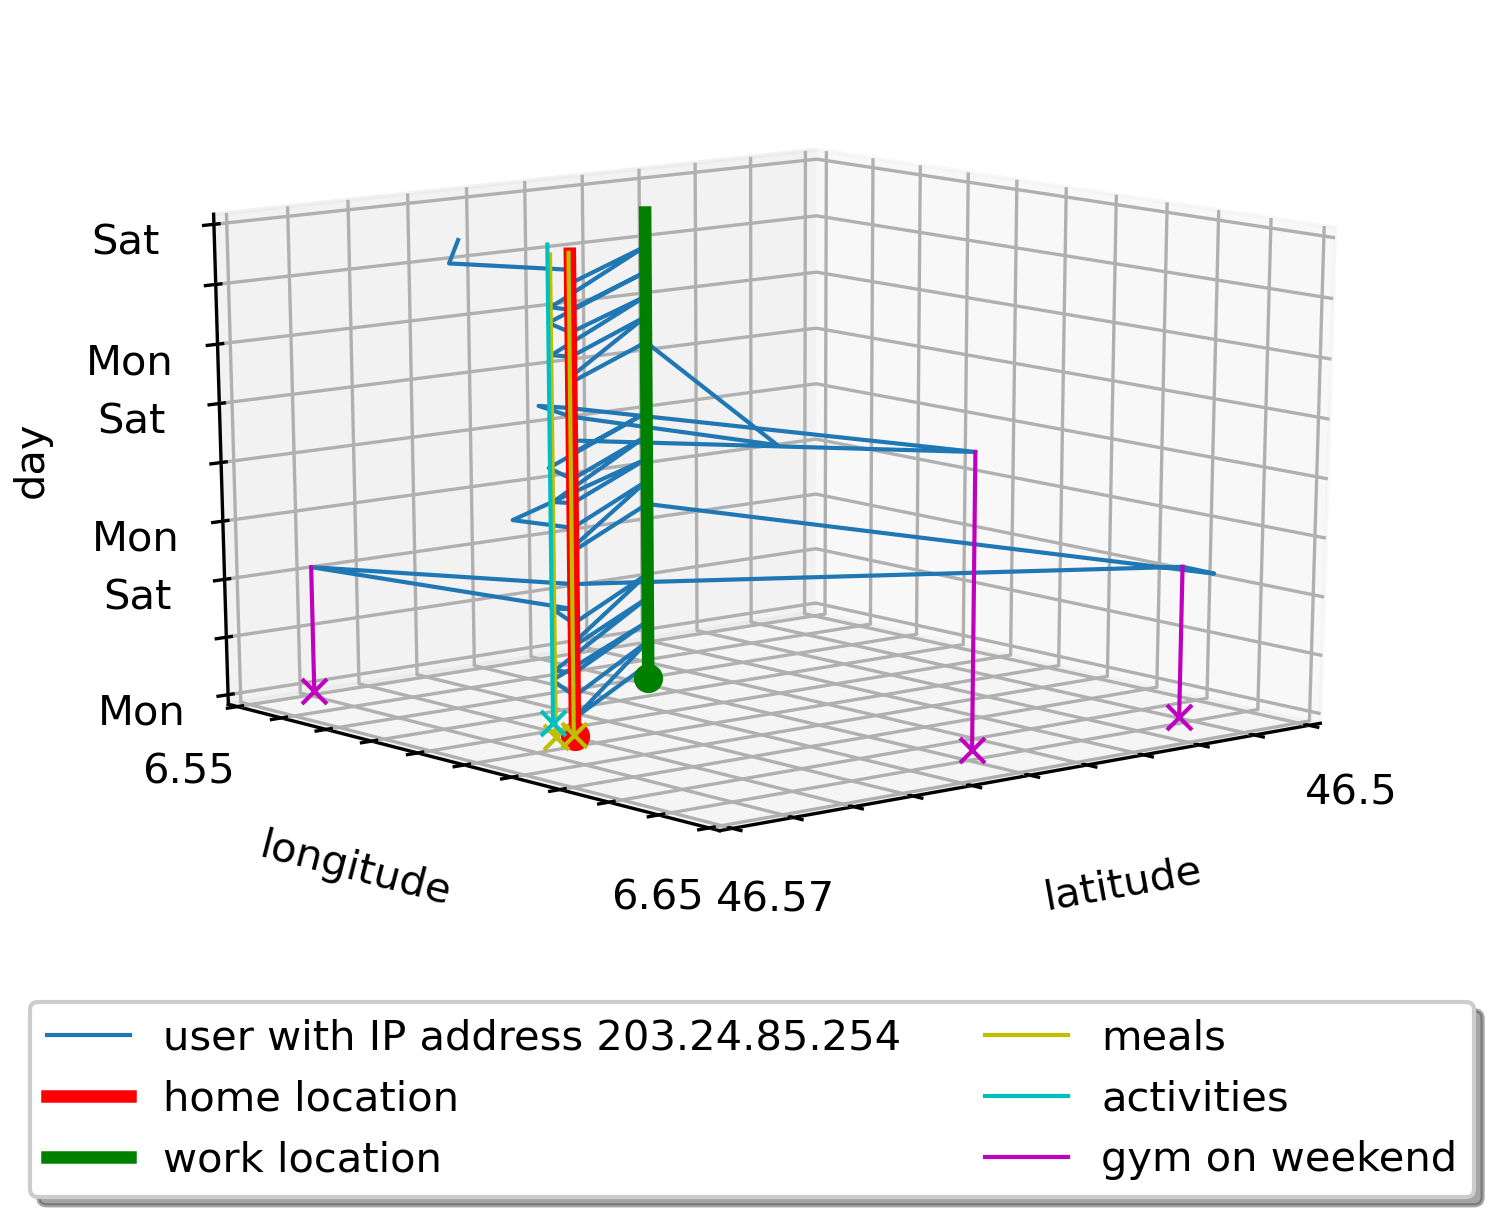
\includegraphics[width=\columnwidth]{random.png}
  \caption{Monitoring of a randomly chosen user using collecting data}
  \label{random_fig}
\end{figure}

\subsection{Defences}
Propose a defence that users of the service could deploy to protect their privacy.  You
should state your assumptions, adversary models, and provide an experimental evaluation of your
defences using the datasets and the grid specification. You should also discuss the
privacy-utility trade-offs of your defence.

\section{Cell Fingerprinting via Network Traffic Analysis}

\subsection{Implementation details}
Provide a description of your implementation here. You should provide details on your data collection methods, feature extraction, and classifier training.

\subsection{Evaluation}
Provide an evaluation of your classifier here -- the metrics after 10-fold cross validation.

\subsection{Discussion and Countermeasures}
Comment on your findings here. How well did your classifier perform? What factors could influence its performance? Are there countermeasures against this kind of attack?

\bibliographystyle{IEEEtran}
\bibliography{bib}
\end{document}
